\section{Development}\label{sec:development}

The development process involved learning many practices
necessary to write a full-stack application.
One of them is splitting the system
into frontend and backend, which
enables easier reuse of the business logic,
and writing different frontend applications
that use the same backend.
Many huge organizations practice splitting
their systems into frontend and backend.
An example of this is Facebook,
which benefits from the ability to use
many different languages and libraries
that can interact between one another~\cite{abdullah_frontend_2014}.

In this section,
I will explain the development of every component
in the Notipie project, which is:
backend,
frontend, and
notification producer.
I will also elucidate the protocol
which is used for communication between aforementioned components,
and I will look into additional programming practices
I used during Notipie implementation.

\subsection{Backend}\label{sec:backend}

The backend is a component in a system
that is responsible for the data processing.
It interacts with the frontend applications
with a well-known protocol,
usually one understood by a browser.

The backend of Notipie
needed to be both performant,
easy to deploy,
and well-tested.
I strived to make use of the best practices
in the field of microservices,
maintain great quality,
and ensure sufficient performance.
I named it \textit{core},
because there can be different \acp{UI},
or notification producers,
but the entire application's core
is specifically the backend implementation.
The backend code
is in the
\texttt{core} directory~\cite{sewera_notipie_2022}.

\subsection{Core project architecture}\label{sec:core-project-architecture}

An overview of the backend architecture
from the asynchronous notification flow perspective
is presented in figure~\ref{fig:high-level-backend-flow}.
The project on the top-level is structured over 4 directories,
named according to
the \citetitle{quest_standard_2022}~\cite{quest_standard_2022}:

\begin{figure}[h]
      \centering
      \includegraphics[width=6.5cm,keepaspectratio]{chart/out/backend-flow.pdf}
      \caption{Backend architecture for asynchronous notification flow}
      \label{fig:high-level-backend-flow}
\end{figure}

\begin{itemize}
      \item
            \texttt{cmd} -- entry point to the application (\texttt{main})
      \item
            \texttt{internal} -- application-specific code
      \item
            \texttt{pkg} -- reusable utils, not specific to the application
      \item
            \texttt{test} -- black box integration test code
\end{itemize}

\subsubsection{The internal directory}\label{sec:the-internal-directory}

Application-specific code is split into 5 directories
representing the levels of abstraction:

\begin{itemize}
      \item
            \texttt{domain} -- business logic,
            defines data structures and communication of domain objects
            on the highest level of abstraction,
      \item
            \texttt{grid} -- lower level of abstraction than domain,
            defines proxies that convert network models into domain models,
            and connects those proxies with the domain components,
      \item
            \texttt{impl} -- implements network endpoints,
            \ac{WS} connections, and persistence,
      \item
            \texttt{infra} -- configures the application
            and sets up the context for \ac{DI}.
\end{itemize}

There also was a \texttt{model} package
in the \texttt{internal} directory,
but I moved it to an exportable \texttt{pkg} directory,
to reuse it in the notification producer.

\subsubsection{Grid}\label{sec:grid}

The grid is an application layer
that connects implementations of
the endpoints, \ac{WS} connections, and persistence
with the domain objects.
I decided to define that name in the \ac{UL}
to mean this exact intermediate layer.
The name itself was inspired by a power grid
which connects components
from power generation
to appliances.

The implementation is based on the proxies
for domain Apps and Users\footnote{
      The App and the User are defined in
      sections~\ref{sec:app}~and~\ref{sec:user}
      respectively.
}.
Those proxies convert the applicable network models
and perform intermediate procedures
that do not concern the domain,
like Notification \ac{ID} generation.

This layer is especially important
to keep the domain clean and concise
and to enable easy replacing\footnote{
      The differences between writing code
      for reuse and replacement are described in detail
      in section~\ref{sec:code-quality}.
}
of concrete implementations.

\subsubsection{Go in core}\label{sec:go-in-core}

Go is quickly gaining popularity among developers,
with its great tooling
and a state-of-the-art standard library.
It is an excellent language for writing microservices.
Its focus on this one task
and pragmatism in adding features to the language by its authors,
resulted in an easy to understand and use,
yet very powerful set of tools.

\paragraph*{Motivation}\label{sec:motivation}

When choosing the right language for the project,
I focused on finding the right tool
for the application and developer experience.

I wanted \texttt{notipie} to be a high-performance microservice,
so I did not take interpreted languages
like Python or \acf{JS} into consideration.
I mostly considered Java, Kotlin, Rust, and Go.

Java, although popular, does not have the greatest developer experience.
Things like \texttt{equals} and \texttt{hashCode}
are unnecessary bloat in the code.
Project Lombok~\cite{zwitserloot_project_2022} fixes some of them,
but the tooling is limited to IntelliJ,
you have to download a lot of libraries for dealing with \ac{JSON},
create your own code style guide,
and perform a fair bit of setup.
Kotlin, far better than Java,
but also locked-in to IntelliJ with tooling,
was an interesting option for me, but not ideal.
Rust was too low-level for my application.
Explicit memory management, although performant,
was simply too verbose and work-intensive for my use case.

Go was a perfect option.
A plethora of great tooling,
like first-party Go plugin for \ac{VSCode}, GoLand from JetBrains,
community plugins for Neovim,
all working great and providing a good developer experience.
Furthermore, extraordinary performance of the tooling itself,
with tests running in under a second, super-fast compiler,
one of the best standard libraries I have seen,
and overall simplicity of the language, made the choice obvious.

\subsubsection{The benefits of using Go}\label{sec:the-benefits-of-using-go}

\paragraph{Built-in language features}\label{sec:built-in-language-features}

There were numerous features
that helped during backend development.
Implicit encapsulation of functions and variables
starting with a lowercase letter,
structure field annotations
enabling easy serialization
to \ac{JSON} and \ac{YAML},
coroutines automatically managed by the Go runtime,
or channels,
just to name a few.
The idea behind most of them
was very simple to understand,
the usage was intuitive,
and I did not have to resort to the documentation that often.

\paragraph{Goroutines and channels}\label{sec:goroutines-and-channels}

Among of the best features of the Go language lay goroutines and channels.
They make concurrent programming a lot easier, compared to other languages.
I used both goroutines and channels
for inter-object communication in \texttt{domain} package.

For example, in {tag.go}~(appendix~\ref{apx:concurrency-in-go}),
after the Tag object is created,
the constructor calls
the \texttt{start} method~(listing~\ref{lst:start-method-in-tag}).
It is running a new goroutine for every Tag instance,
enabling them to asynchronously communicate with other objects.

The Tag was a particularly special case,
in which I had to solve
the Notification duplication problem,
described in detail in section~\ref{sec:tag-technicalities}

\paragraph{Standard library}\label{sec:standard-library}

Standard \texttt{testing} package~\cite{cox_testing_2022} provided
a unified, and simple tooling for testing.
I did not have to think anything about test setup.
No custom scripts, third-party libraries, or \ac{IDE} setup.
All I needed to do was to name a file with a \texttt{\_test.go} suffix,
write a function starting with \texttt{Test},
and run \texttt{go\ test\ ./...}.
Both \ac{VSCode} with Go plugin and GoLand
automatically picked up the test setup,
and I was ready to develop with \ac{TDD}.

Standard \texttt{net/http} package~\cite{cox_http_2022} provides everything
needed for setting up \ac{REST} endpoints.
Although I used Gin~\cite{martinez-almeida_gin_2022} for this,
due to a simpler interface,
I used status codes
and \ac{HTTP} client implementation
from \texttt{net/http}.

\paragraph{Refactoring to the standards}\label{sec:refactoring-to-the-standards}

During this project,
I refactored my functions to better suit
the Go standard library.
It was beneficial
not only because of a better integration
with the standard library itself,
but also because of a better integration
with third-party libraries.
There is an unwritten rule,
that every library strives
to be as compatible
with the standard library as possible.

For instance,
in commit \texttt{00547cd}\footfullcite{sewera_chorecoreproducer_2022},
I refactored the \texttt{ToJSON} method
to better suit the standard signatures
(appendix~\ref{apx:method-signature-refactoring-in-go}),
i.e. to return the byte array and error,
just like the \texttt{Marshal} method
from the \texttt{json} package~\cite{cox_json_2022}
in the standard library.

\paragraph{Third-party libraries}\label{sec:third-party-libraries}

Gin was great for writing \ac{REST} endpoints,
with \texttt{gin.Context} having easy access to
standard-library-compatible fields,
making it easily pluggable to other third-party libraries,
like Gorilla WebSocket~\cite{burd_gorilla_2022}.

Zap~\cite{shah_zap_2022} provided a reliable
and performant way to log things in the backend.
Structured logging,
straightforward syntax,
automatic serialization to \ac{JSON} in production mode,
and human-readable format in debug mode,
paired with low or zero-allocation overhead,
made it a perfect choice for logging in a microservice.

\addtocategory{commit}{sewera_chorecoreproducer_2022}


\subsection{Frontend}\label{sec:frontend}

The frontend's purpose is to present the data
it got from the backend to a user
in a manner that is both easy to read
and visually attractive.
Modern frontend applications
are expected to include
fast loading times,
asynchronous data fetching,
intuitive interface,
and some degree of familiarity,
which means they have to resemble
popular services to some extent.

When designing the \ac{UI} for Notipie,
I wanted not only to deliver great visual design,
but also intuitive user experience,
reliability,
and snappiness.
The frontend code
can be found in the
\texttt{ui} directory of the Notipie project~\cite{sewera_notipie_2022-5}.
The \ac{UI} is available both in dark and light mode,
as illustrated in figures~\ref{fig:notipie-ui-dark}
and~\ref{fig:notipie-ui-light} respectively.

\begin{figure}[h]
  \centering
  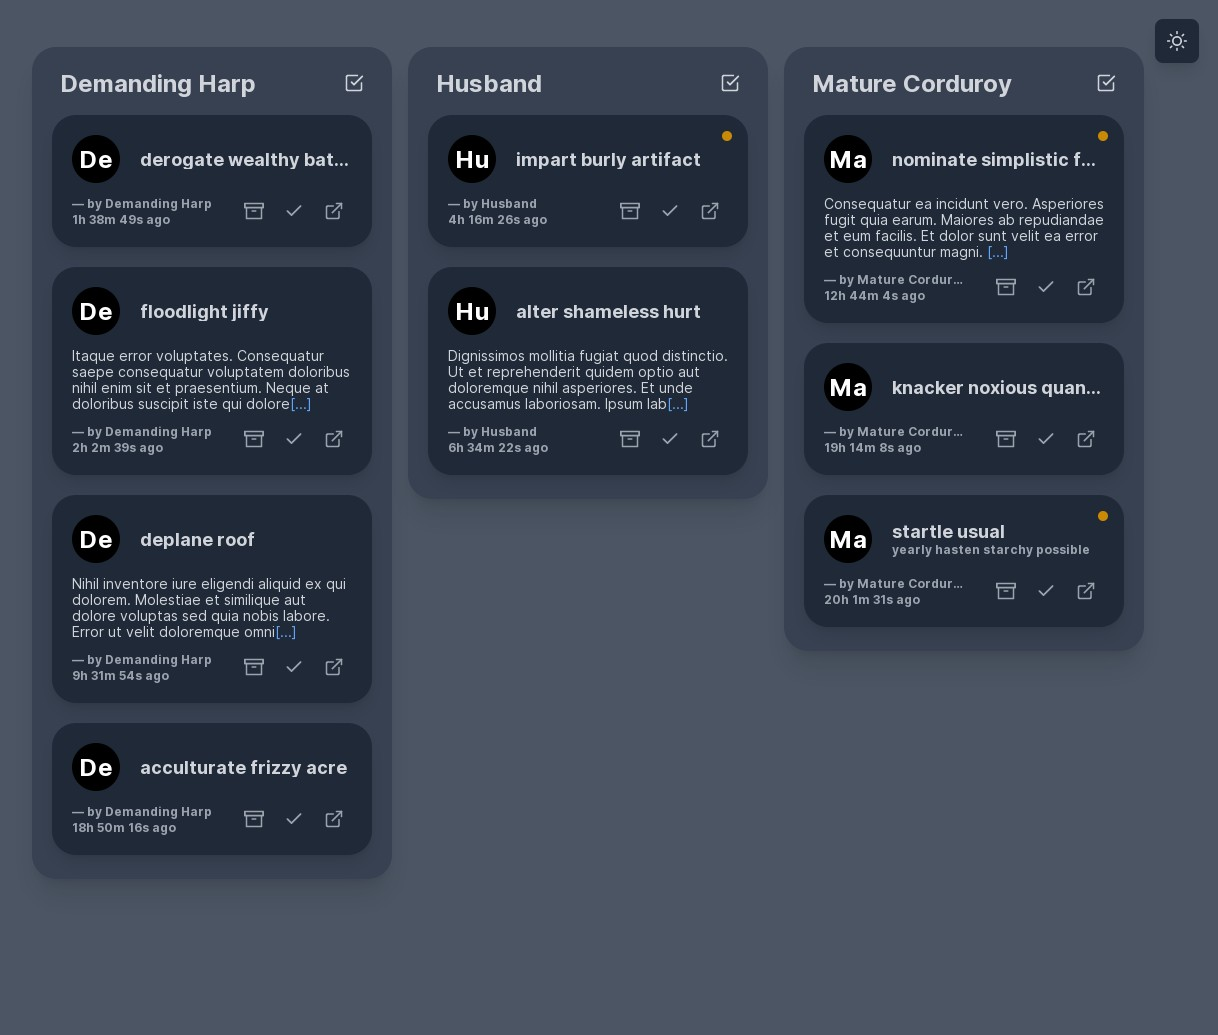
\includegraphics[width=9cm,keepaspectratio]{img/notipie_dark.jpg}
  \caption{Notipie UI: Dark mode}
  \label{fig:notipie-ui-dark}
\end{figure}

\begin{figure}[h]
  \centering
  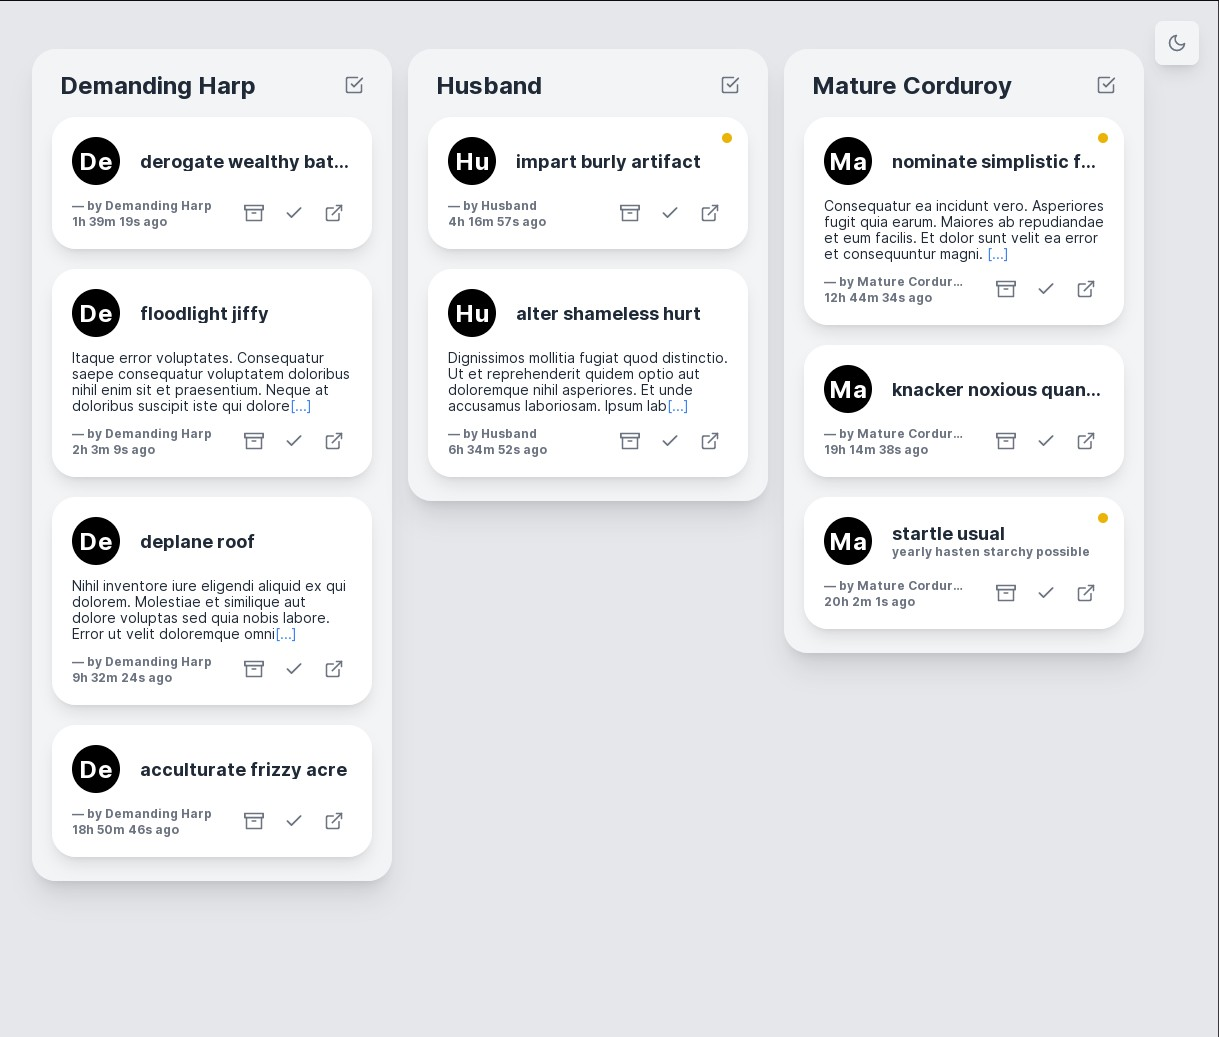
\includegraphics[width=9cm,keepaspectratio]{img/notipie_light.jpg}
  \caption{Notipie UI: Light mode}
  \label{fig:notipie-ui-light}
\end{figure}

\subsubsection{UI Design}\label{sec:ui-design}

When designing the \ac{UI} of Notipie,
I tried to maximize usability
and minimize complexity of the interface.
Maintaining simplicity of the interface is not an easy task,
so I took inspiration from the professional designs.

\paragraph*{Inspirations}\label{sec:inspirations}

My main inspirations for the interface included
Apple Human Interface Guidelines~\cite{apple_inc_human_2022}
and Google's Material Design~\cite{google_llc_material_2022},
but by far the most inspiration was taken from
Github Primer~\cite{github_inc_primer_2022}.
I tried to break down what is useful,
what is unnecessary in my project,
and extract only the essentials for my design.
I began designing with freehand sketching
on my e-book (figure~\ref{fig:early-ui-sketches}).
It allowed me to quickly visualize my ideas
and decide on the elements that I like.

\begin{figure}[h]
      \centering
      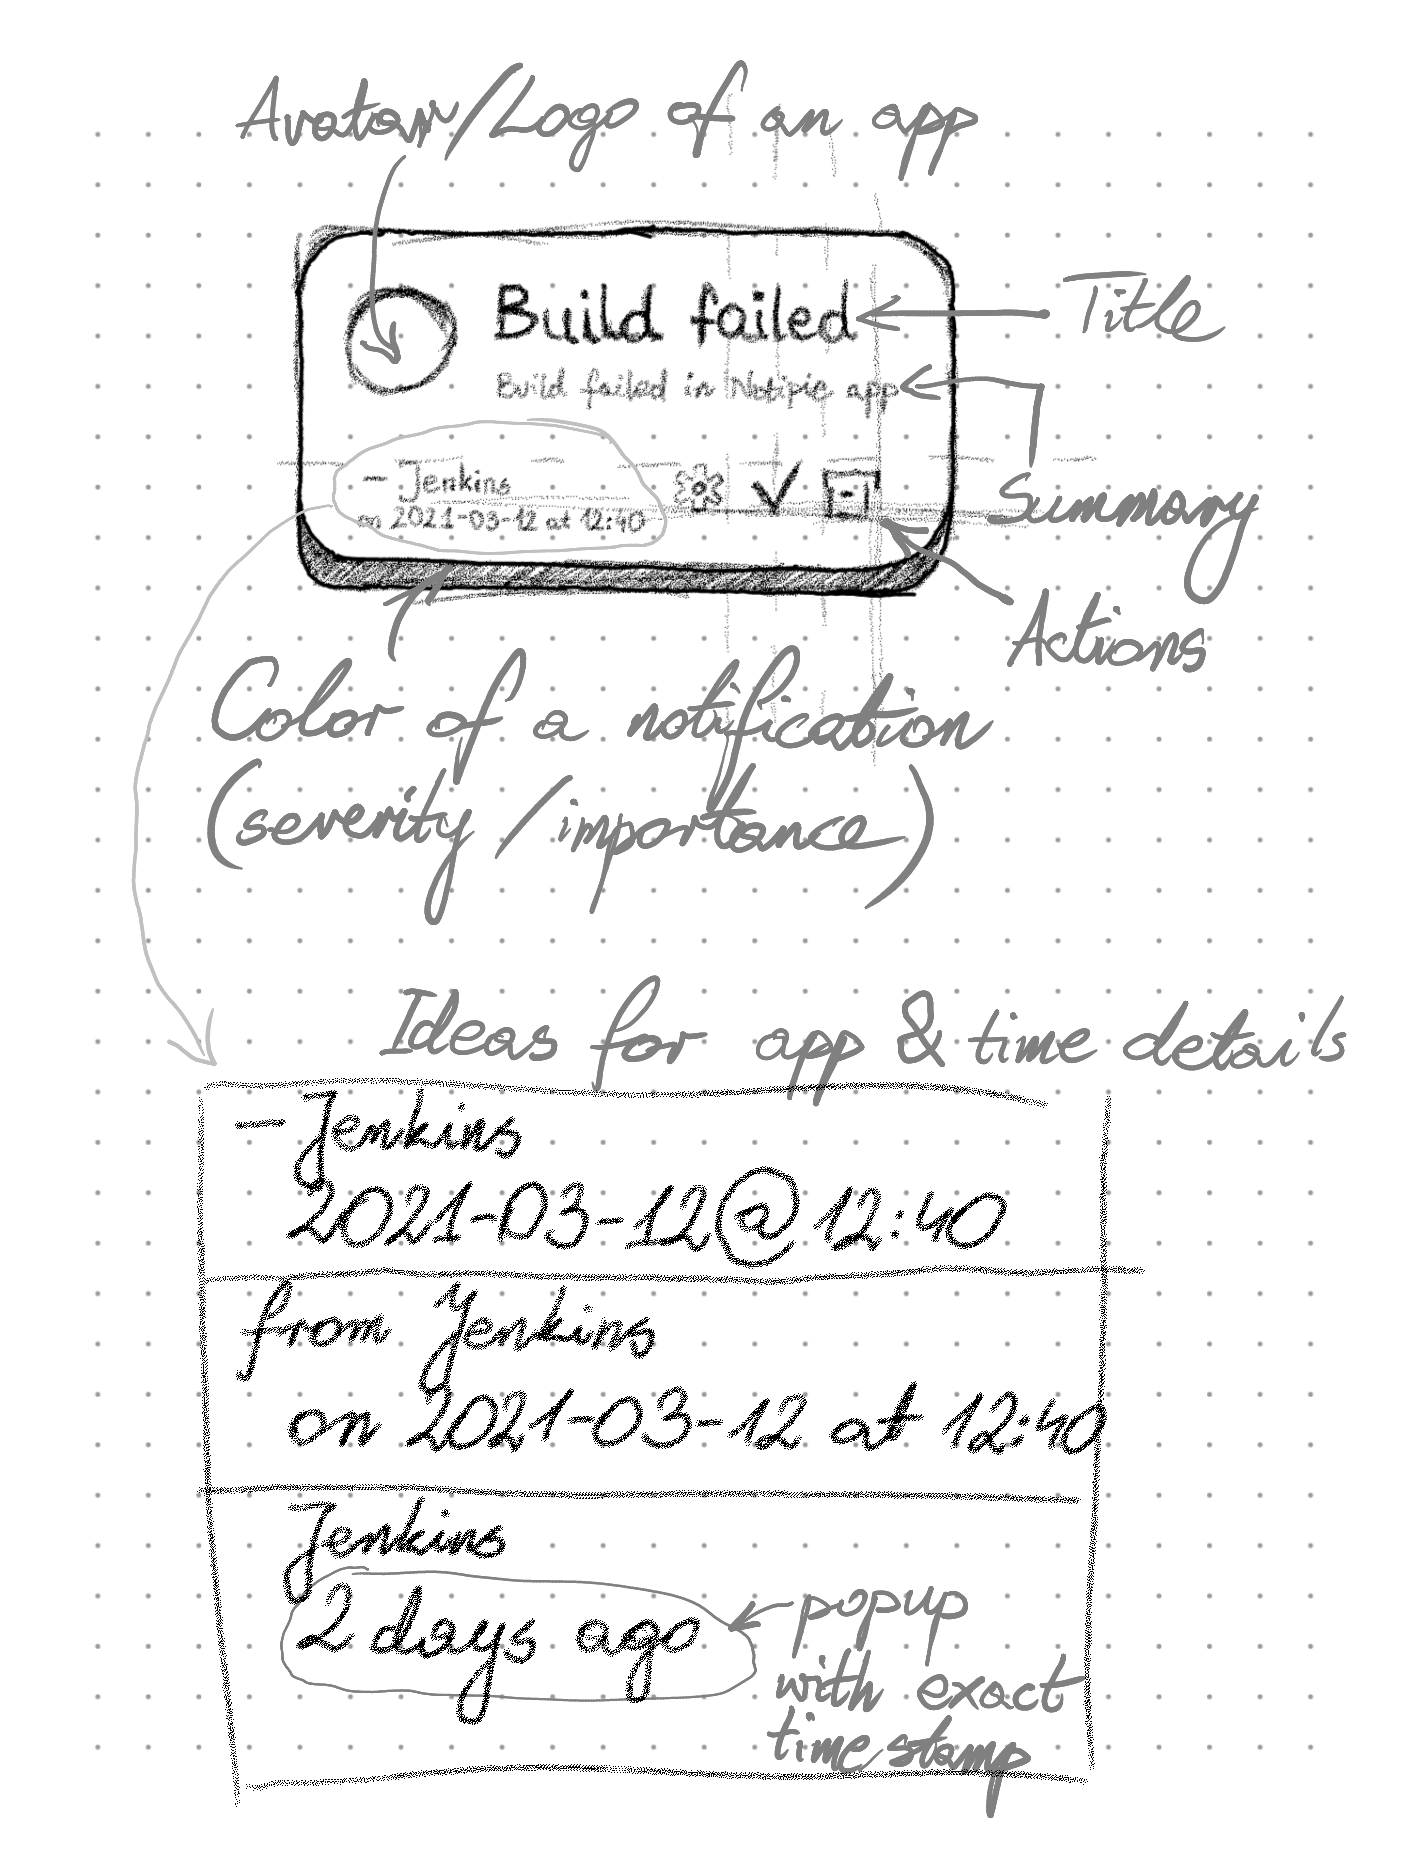
\includegraphics[width=10cm,keepaspectratio]{img/early_ui_sketches.png}
      \caption{Example early sketch made on e-book}
      \label{fig:early-ui-sketches}
\end{figure}

The works of Adam Wathan and Steve Schoger
also had a great influence
on my design decisions.
Their book,
\citetitle{wathan_refactoring_2018}~\cite{wathan_refactoring_2018}
was an excellent guidance on best practices
of modern \ac{UI} design.

\paragraph*{Final design}\label{sec:final-design}

The card is a building block for the entire \ac{UI}.
It provides the most interaction in the whole application,
therefore it had to be designed with a clear information layout
and intuitive controls.
The card itself consists of several elements,
as depicted in figure~\ref{fig:card-with-labeled-elements}:

\begin{enumerate}
      \item
            logo,
            it can be an image
            or automatically generated \ac{SVG}
            from the first two letters of the app's name,
      \item
            indicator,
            whether the notification has been seen or not,
      \item
            title of the notification,
      \item
            subtitle,
      \item
            body,
            which collapses after it reaches a certain length,
            so that an ellipsis appears (\texttt{...}),
      \item
            information about what app sent the notification and when it happened,
      \item
            controls to archive,
            mark as read,
            or go to external site connected with the notification,
            like a certain build on Jenkins,
            or the notification page on Github.
\end{enumerate}

The card was also designed with aesthetics in mind.
All elements were carefully positioned and aligned,
so they are not only pleasant to look at,
but also have features important for visual communication.
Those features, highlighted in figure~\ref{fig:card-with-guides}, include:

\begin{itemize}
      \item
            the rounded corners take the focus away from the card frame,
            and provide a natural, neutral enclosure for the notification,
      \item
            the inner padding is of equal size in each direction
            to provide optical stability,
      \item
            the distance between the logo and title -- subtitle combo
            is the same size as the padding,
            making the logo appear centered,
      \item
            the title -- subtitle combo itself
            is centered vertically relative to the logo,
      \item
            the distances between the logo,
            notification body, and app name -- timestamp combo are shorter
            in order to make the inner section more connected,
      \item
            the controls are centered relative to the app name -- timestamp combo,
      \item
            the \textit{unread} indicator is unobtrusive enough
            not to steal all the focus from the card's content,
      \item
            finally, the \textit{unread} indicator
            is positioned slightly outside the inner section,
            so that it belongs to the card itself,
            not its content,
            therefore it is easier to spot at a glance.
\end{itemize}

\begin{figure}[p]
      \centering
      \begin{minipage}{0.45\textwidth}
            \centering
            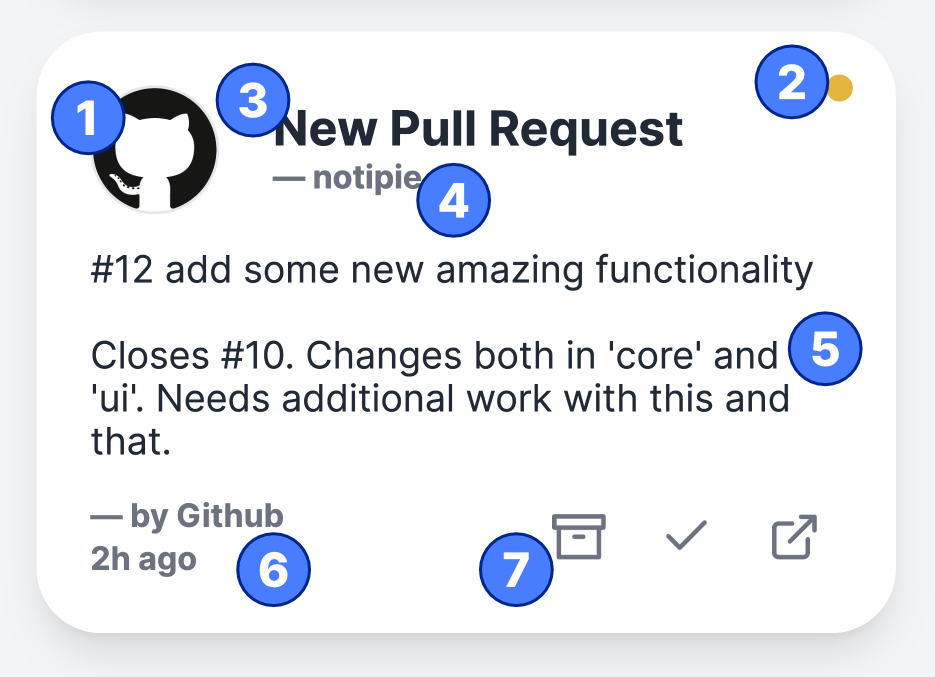
\includegraphics[width=0.9\textwidth,keepaspectratio]{img/card_labeled.png}
            \caption{Card with labeled elements}
            \label{fig:card-with-labeled-elements}
      \end{minipage}\hfill
      \begin{minipage}{0.45\textwidth}
            \centering
            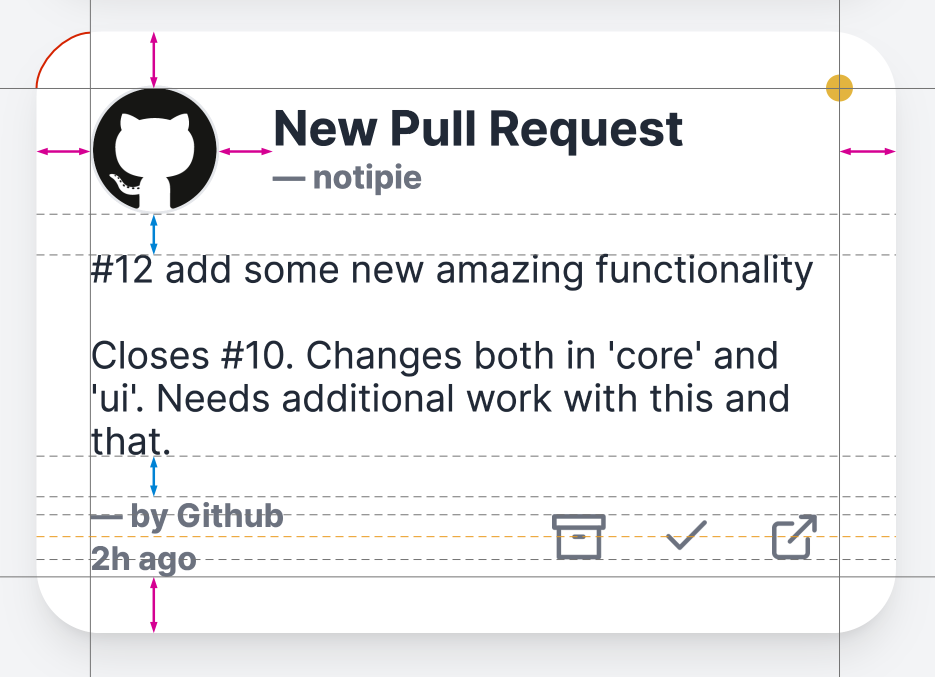
\includegraphics[width=0.9\textwidth,keepaspectratio]{img/card_guides.png}
            \caption{Card with guides}
            \label{fig:card-with-guides}
      \end{minipage}
\end{figure}

\subsubsection{UI components}\label{sec:ui-components}

Using components enabled me to split my \ac{UI}
into small, reusable components,
eliminating code duplication,
and helping maintain consistent look.
I wanted to choose the right library
for this task,
so that the development would be quick,
and I would have plenty of tools
that would help me achieve
good architecture for the frontend.

\paragraph*{UI component library}\label{sec:ui-component-library}

A \ac{UI} component library is a \acf{JS} or \acf{TS} library
enabling a programmer to reduce duplication
in the frontend codebase.
It provides a way to split the frontend code into components,
which can be parametrized, reused, and composed into an entire application,
and to declaratively describe
the appearance and behavior of those components
with a~help of functions or classes.
When choosing the library for the \ac{UI} components, I~considered:

\begin{itemize}
  \item
        React~\cite{oshannessy_react_2022},
  \item
        Vue.js~\cite{you_vuejs_2022}, and
  \item
        Angular~\cite{kalpakas_angular_2022}.
\end{itemize}

All those libraries are very popular,
so I chose React,
because I had the most experience with it in my professional work.

\paragraph*{The component directory}\label{sec:the-component-directory}

All of the frontend components
are located in the component directory~\cite{sewera_notipie_2022-3}.
The directories are divided by category.
There are currently two categories,
\textit{canvas}, and
\textit{notification}.
Canvas category includes
an \texttt{AppCanvas} component,
which is responsible for displaying
a background in the right color,
and controlling the light or dark mode setting.
Notification category includes
a notification card,
a notification container,
which contains all the notifications
from the same App\footnote{
  The concept of an App is described
  in section~\ref{sec:app}.
}, and a notification board,
containing all the notifications
presented in the \ac{UI}.

\paragraph*{Styling}\label{sec:ui-styling}

In addition to the correct behavior of the \ac{UI},
I needed to bring my design of the card\footnote{
  The design of the card
  is explained in detail
  in section~\ref{sec:final-design}.
} and other components
into reality.
I had some experience with Bootstrap~4~\cite{otto_bootstrap_2018},
but I did not like the look of it,
and on top of that,
customizability was complicated.
I also had experience with plain \ac{CSS},
but I did not want additional hassle
of maintaining both \ac{JS} and \ac{CSS}.

I decided I will use a \ac{CSS} utility library,
which will remove additional effort
of manual \ac{CSS} management,
as well as provide me with the necessary tools
to implement my own, custom design.
Tailwind~CSS~\cite{wathan_tailwind_2022}
was my first and only choice.
Not only is it very popular,
but also the documentation is excellent,
there are many tutorials on YouTube,
and it was written by the authors
of \citetitle{wathan_refactoring_2018}~\cite{wathan_refactoring_2018},
one of the books that influenced
my style of design overall,
mentioned also in section~\ref{sec:inspirations}.

\paragraph*{Testing}\label{sec:ui-testing}

\Ac{UI} visual testing tends to be very expensive,
both in terms of time and money.
I used Applitools Eyes~\cite{applitools_applitools_2022}
in my professional work,
and it was both slow,
and the tests were flaky.
I also did not want to spend any money
on the application development.

I used Jest~\cite{bekkhus_jest_2022} for unit tests,
and I was very content with it.
I found out that it has
a \textit{snapshot testing} capability~\cite{bekkhus_snapshot_2022}.
In addition to a \ac{CSS} utility library
like Tailwind~CSS,
I could be fairly sure
that if all \ac{HTML} classes stayed the same,
the look of the entire application
will stay the same.

The snapshot tests were very quick
and easy to review.
The were also easy to debug,
whenever there was some unwanted change.
Coupled with Tailwind~CSS,
they provided a very powerful tool
for regression testing.

\paragraph*{Storybook}\label{sec:storybook}

Another tool that helped with
component creation in isolation
was Storybook~\cite{shilman_storybook_2022}.
The isolation of components
helped with testing,
improved portability and reusability,
and helped me gather all the properties
of each component into an interactive
documentation.
It provided a convenient component library browser,
which worked both in dark and light mode.
The Storybook for Notipie is presented
for dark and light modes in
figures~\ref{fig:storybook-dark}
and~\ref{fig:storybook-light}
respectively.

\begin{figure}[hp]
  \centering
  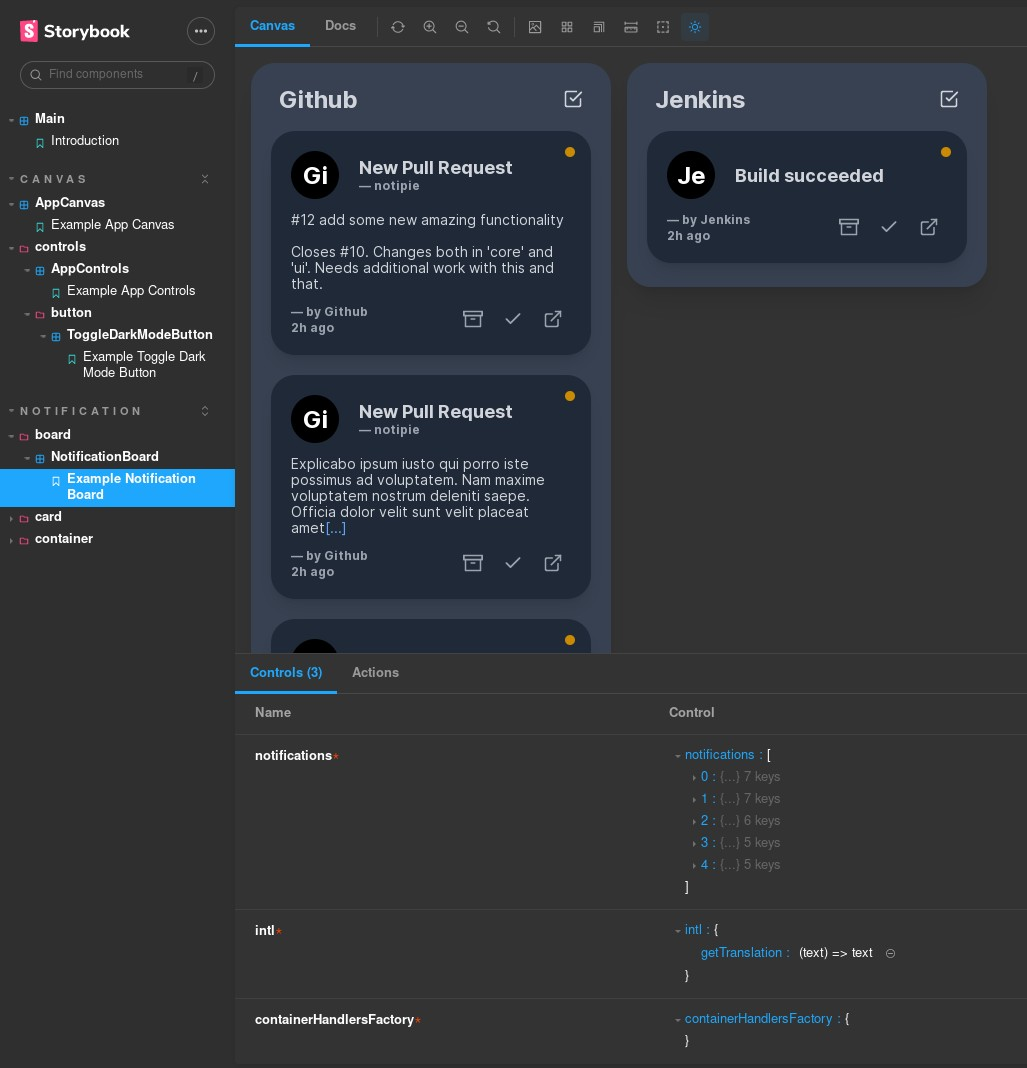
\includegraphics[width=\linewidth,keepaspectratio]{img/storybook.jpg}
  \caption{Storybook for Notipie: Dark mode view}
  \label{fig:storybook-dark}
\end{figure}

\begin{figure}[hp]
  \centering
  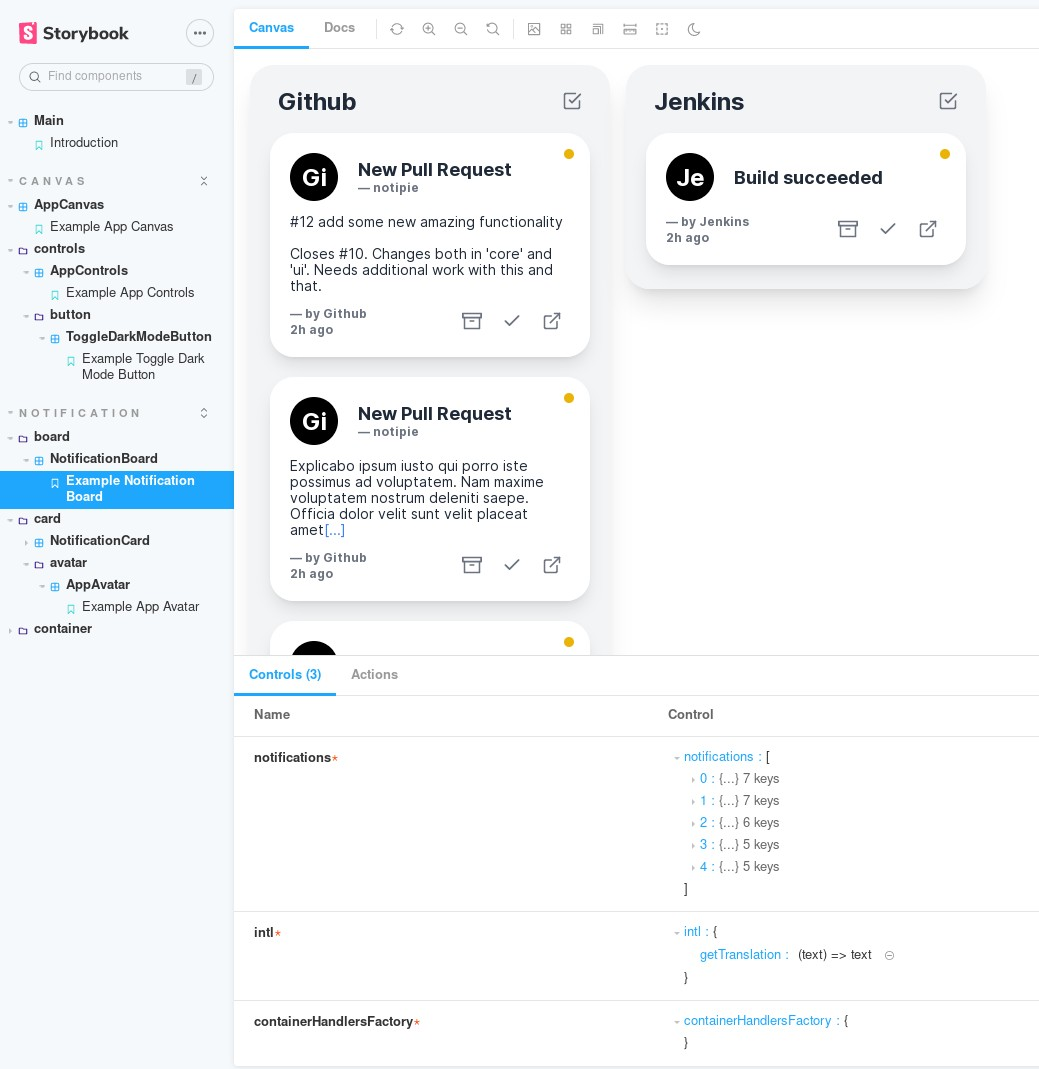
\includegraphics[width=\linewidth,keepaspectratio]{img/storybook_light.jpg}
  \caption{Storybook for Notipie: Light mode view}
  \label{fig:storybook-light}
\end{figure}

\subsubsection{UI networking}\label{sec:ui-networking}

The nature of notifications required me to use
both \ac{REST} data fetching and asynchronous data pushes from the backend.
For the latter, I decided to use \ac{WS},
a standard defined in RFC6455~\cite{fette_rfc6455_2011}, and
RxJS~\cite{lesh_rxjs_2022}, an implementation of
ReactiveX library~\cite{gross_reactivex_2021}.

\paragraph*{REST data fetching}\label{sec:rest-data-fetching}

I used simple \ac{REST}~\cite{perrier_rest_2022} requests
for fetching the notifications
that are already on the backend server.
The standard Fetch browser \ac{API}~\cite{perrier_fetch_2022}
was sufficient for the task.

\paragraph*{Reactive Raven}\label{sec:reactive-raven}

This project~\cite{sewera_reactive_2022} was an experiment
on using RxJS for all real-time data fetching,
enabling the separation of concerns in the code,
and decoupling the state management implementation
from the networking implementation.
When searching for the optimal solution
for pushing the data to the \ac{UI},
I came across two major solutions:

\begin{itemize}
      \item
            Redux Thunk~\cite{gaeraon_redux_2022-1} --
            enough for fetching data on user interaction,
            e.g., on a button click,
            but it provides virtually full implementation lock-in
            to the Redux store, and very little separation of concerns.
            Fetching data is an action dispatched on a store,
            so external communication and storing data are dependent on each other.
      \item
            Redux Saga~\cite{elouafi_redux_2022} --
            good for managing side effects with plain \ac{JS},
            but it uses generator functions
            that yield a different type every time,
            so it is very problematic to use with strict \ac{TS}.
\end{itemize}

Unfortunately,
Thunks and Sagas did not provide the separation of concerns
I wanted to achieve.
Fetching or acting upon pushed data
is a different concern than storing it.
Both had a strict dependency on Redux
store implementation,
so I discarded them as an unacceptable risk
of relying on libraries I could not change.

As a user,
I should not have to dispatch an action on a store
when I want to fetch data.
Of course, the data can be immediately stored after fetching,
but this behavior should be injected later,
so that there is no store implementation lock-in.
The separation of concerns created by using RxJS
enabled me to migrate from Redux to Zustand
as my store implementation,
as described in the next section.

\subsubsection{State management in UI}\label{sec:state-management-in-ui}

To simplify the frontend code,
I needed to use a single source of truth for the data.
Store,
which is a solution for state management
in frontend applications,
is~a~Singleton~\cite{gamma_design_1994}
that can be read by any component,
but can be mutated only using certain functions,
or, in Redux library's case, dispatching actions.
This~approach prevents any data races
or having the store in an unstable state.
I~used both Redux~\cite{gaeraon_redux_2022},
and Zustand~\cite{kato_zustand_2022} for this task
as store implementations,
and Zustand came on top as a simpler solution for my application.

\paragraph*{Redux}\label{sec:redux}

Redux is great for big applications with lots of components.
Being one of the most popular state management libraries for React,
it was my first choice.
Unfortunately,
it required me to write a lot of boilerplate code,
and thus was not easily maintainable
for a smaller project like Notipie.

\paragraph*{Zustand}\label{sec:zustand}

Zustand is a lot simpler than Redux,
requires a lot less boilerplate code,
and was sufficient for my application.
I migrated to it in commit
\texttt{7677d13}\footfullcite{sewera_choreui_2022},
and it reduced the lines of code by over 200.
I did not, however, give up the connected components,
as they provide better testability and separation of concerns,
which is worth a bit extra code.

\addtocategory{commit}{sewera_choreui_2022}

\subsubsection{TypeScript in UI}\label{sec:typescript-in-ui}

There are many tools that can help with maintaining
a frontend codebase.
Linters,
static checkers,
or libraries enforcing certain type at runtime,
just to name a few.
For many years,
we had no other choice but to use
\ac{JS} in frontend projects.
\Acl{TS} is by far the most valuable tool that helps
with making the code maintainability easier.
I decided to use it in my project for the frontend part,
because of its type checking tools,
huge popularity,
and a growing demand for it on the job market.

\paragraph*{Choosing the language}\label{sec:choosing-the-language}

When choosing which language to use in the \ac{UI},
I considered a couple of options:

\begin{itemize}
  \item
        plain \acl{JS},
  \item
        \acl{TS},
  \item
        Elm, and
  \item
        CoffeeScript.
\end{itemize}

I immediately discarded the last two
due to their smaller popularity,
compared to \acl{JS} or \acl{TS}.
Elm and CoffeeScript may have seen
a spike of popularity before \acl{TS}
became main stream,
but as of today,
they have a minuscule market share.

The feature set of the language was also very important to me.
\Acl{JS} is by far the most popular,
but it lacks type annotations or pre-runtime type checking.
\Acl{TS} and Elm turned out to be winners in the type checking toolchain.
\Acl{TS} also has a big advantage of being very similar to plain \acl{JS},
so the transpiled code is very readable.

A big factor was general trend of language's popularity growth.
\Acl{TS} was a clear winner in this scenario,
being third most loved language
and second most wanted language
in the Stack Overflow Developer Survey 2021~\cite{stack_overflow_2021_2021}.
It was only beaten by Rust and Clojure
in the \textit{Most Loved} section,
both of which are non-frontend languages,
and Python in the \textit{Most Wanted} section,
which is also not a frontend language.
Another report confirming the growing popularity of \acl{TS}
is Github Octoverse Report 2021~\cite{github_inc_2021_2021}.
Since 2017,
it beat
Ruby,
C,
C++,
C\#,
Shell, and
\ac{PHP}
and is, as of 2021, the fourth top language on Github.

\paragraph*{Working with TypeScript}\label{sec:working-with-typescript}

Starting with \acl{TS} was fairly easy.
The toolchain was included in the project creation scripts.
Most dependencies had good \acl{TS} annotations,
or they were completely written in \acl{TS},
which was very helpful for maintaining type safety.

Learning the language was also very easy.
I was already familiar with \acl{JS},
so I only needed to learn
the syntax of type annotations,
which were very intuitive to use.
I also found out that because of the type annotations,
function composition became much easier,
so I had less problem working with more complex
language structures.
\Acl{TS} made writing code easier than \acl{JS}.

\subsubsection{Build system}\label{sec:build-system}

For the build and bundle software,
I wanted to use something modern,
with hot module reloading,
easy to use setup scripts,
customizable development server,
and short bundle times.
One library I immediately ruled out
because of lack of those modern features
was Webpack~\cite{koppers_webpack_2022}.
It is a tool with a lot of legacy,
which brought \ac{JS} bundling to the main stream.
However, today its legacy gets in the way
of a clean \ac{API} and good developer experience,
compared to more modern tools.

\paragraph*{Snowpack and Vite}\label{sec:snowpack-and-vite}

I started with Snowpack~\cite{schott_snowpack_2021}
and used it until I decided to move to Vite~\cite{you_vite_2022}
in commit \texttt{c11bc35}\footfullcite{sewera_choreui_2021}.
Snowpack offered both hot module reloading and short bundle times.
Nevertheless,
there were some minor glitches and bugs from time to time,
the project had a slow development,
small user base,
and the alternative, Vite,
did not seem to have those problems.

I tried Vite in my other project,
Reactive Raven~\cite{sewera_reactive_2022},
and the integration with
React,
\ac{TS},
Tailwind~CSS,
and other tools I used was seamless,
therefore I decided to migrate to it in Notipie as well.
On April 20th, 2022,
Snowpack's maintainer stated in the project's Readme document
(commit \texttt{45456aa}\footfullcite{schott_readmemd_2022})
that he would no longer maintain the project,
and mentioned Vite as a good alternative for it.

\addtocategory{commit}{sewera_choreui_2021,schott_readmemd_2022}


\section{Producer}\label{sec:producer}

The notification producer for Notipie
needed to be easy to use for developers
and system administrators.
Therefore,
I decided to provide both a Go library,
and a command line utility
that can easily be run on all major platforms
and operating systems.
The notification producer code
is in the
\texttt{producer} directory~\cite{sewera_notipie_2022-4}.

\subsubsection{Go library}\label{sec:producer-go-library}

In order to make the notification producer
accessible to developers,
I created a~simple Go library
for easy notification creation and sending.
The library supports the basic operations
an App\footnote{
  The App is defined in section~\ref{sec:app}.
}, or rather its equivalent outside of the domain,
can~perform.
Those operations include pinging
the backend to check if it is up,
and pushing the notification to the backend.

The first operation is useful when setting up
a producer that can push to different backends,
depending on which one is up.
For example,
two backends are running
in two different VPNs.
Depending on which one of them
the computer producing notifications
is connected to,
it first pings those two,
and decides on which one to send the notification to.
This operation can be performed
when starting the producer up,
without the need to send a real notification.

Pushing the notification to the backend
also includes getting the App \ac{ID} from the backend.
The App \ac{ID} is generated whenever
a new App object in the domain is created
(section~\ref{sec:app}).

\subsection{Command line utility}\label{sec:command-line-utility}

Not everyone who could benefit
from my application
needs to have a good understanding
of Go development.
That is why I also prepared
a command line utility
that is compatible with the most popular shells:
Unix-like shells and Powershell.

Its feature set is very similar
to the one mentioned in the previous section,
but it also includes configuration
and notification templates
for convenience.
This in turn enables its users
to set up the producer for multiple Apps
on one system.
It is only necessary to provide
separate configuration files
and, optionally, separate notification templates.
An example of such setup is presented
in figures~\ref{fig:notipie-one-notification}
and~\ref{fig:notipie-two-notifications}.

\subsubsection{Configuration and notification templates}\label{sec:configuration-and-notification-templates}

This version of a producer can be configured
either through the command line arguments,
or the configuration files,
but the command line arguments
always take precedence.
The configuration files themselves
can be stored in \ac{JSON} or \ac{YAML} format.
I chose those two,
because they are very popular formats
for this use case.
Those formats can also be used
for specifying a notification template.

The configuration consists of
the address and port of the backend,
which are set by user.
Also, when the producer sends its first notification
and gets back the App \ac{ID},
the producer appends it to the configuration file,
so that it is present in every consecutive push.

The notification template can be any
subset of an App notification model
defined in section~\ref{sec:protocol}.
Everything specified in this template
can be overwritten with \ac{CLI} arguments.
The only requirement for a valid request
is to have an App name and title set.
The timestamp is set automatically for us.

\subsubsection{Usage}\label{sec:producer-usage}

As described in the previous section,
the producer allows different configurations
for one \ac{CLI} program,
enabling user to set up many different Apps
on the same computer.
Figures~\ref{fig:notipie-one-notification}
and~\ref{fig:notipie-two-notifications}
show the producer sending the notifications
to the Notipie \ac{UI}.
The producer is executed
with different configurations
and notification templates.
The configurations only differ
with the randomly-generated App \ac{ID}.

\begin{figure}[p]
  \centering
  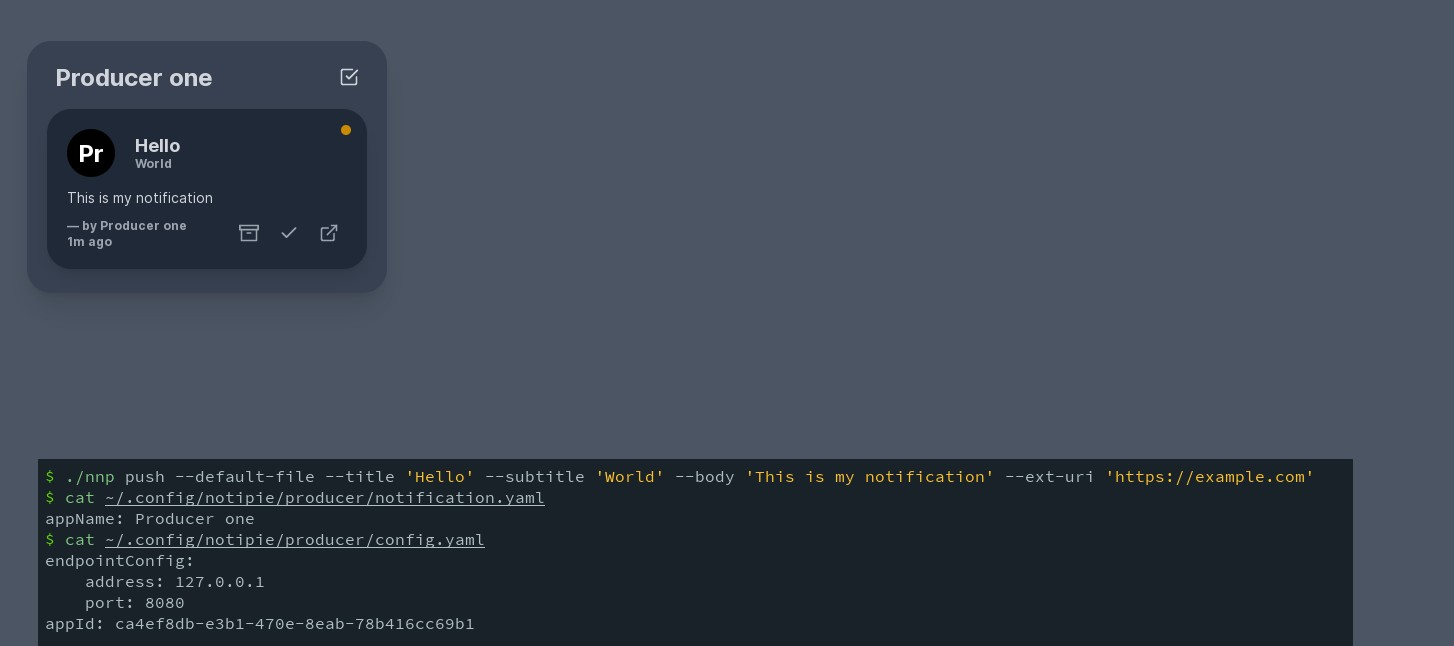
\includegraphics[width=\linewidth,keepaspectratio]{img/notipie_one_notification.jpg}
  \caption{First producer pushing a notification to the UI}
  \label{fig:notipie-one-notification}
\end{figure}

\begin{figure}[p]
  \centering
  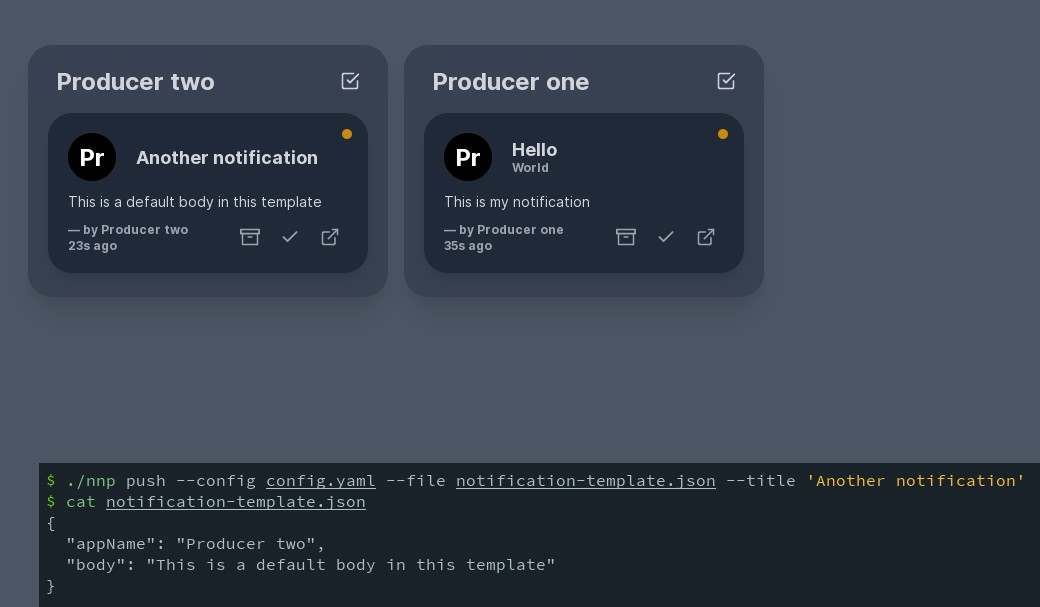
\includegraphics[width=\linewidth,keepaspectratio]{img/notipie_two_notifications.jpg}
  \caption{Second producer pushing a notification to the UI}
  \label{fig:notipie-two-notifications}
\end{figure}


\section{Protocol}\label{sec:protocol}

The Notification\footnote{
  The Notification is defined in section~\ref{sec:notification}.
} in the terms of a domain
was not suitable for the communication
between the producer, backend, and frontend.
That is why I specified a network protocol
for sending notifications
and replying with App \ac{ID} to a producer.
I needed to choose the right format
and develop a set of fields
containing all the useful information.

\subsubsection{Format}\label{sec:protocol-format}

When I was choosing the right format
for the notifications,
I took into consideration two options:
binary and plain text.
I chose plain text,
because portability was very important to me.
I wanted to have the protocol able to run
between different processor architectures,
and not think about endianness.

Then, I wanted to use a format
that was popular for network data exchange.
The candidates were \ac{XML} and \ac{JSON}.
I did not want to go with \ac{XML},
as the parsing is not that easy,
readability is very poor,
and the popularity is dropping
in favor of \ac{JSON}.
I chose \ac{JSON}
because of its support by \ac{TS} and Go,
either as a language feature,
or in a standard library.
I also chose \ac{JSON} for the push response
containing App \ac{ID}
for consistency.

I decided to support both \ac{JSON} and \ac{YAML}
in the configuration files for the producer,
including the notification template\footnote{
  More on the configuration files and templates
  for the producer
  in section\ref{sec:configuration-and-notification-templates}.
}.
\ac{YAML} is favorable in configuration files,
so I wanted to provide a uniform
format for a configuration file
and a template.
\ac{YAML}, however,
does not go through the network
anywhere in Notipie.

\subsubsection{Fields}\label{sec:protocol-fields}

I created two versions of notification models.
One for the App,
and one for the client\footnote{
  A client is, e.g.,
  a browser tab running Notipie \ac{UI},
  and is represented
  by a User in the domain (section~\ref{sec:user}).
}.
They have a common subset of fields,
named \texttt{HashableNetNotification}.
\textit{Hashable},
because this portion is hashed with 256-bit \ac{SHA-2}
in order to generate a unique notification \ac{ID}.
The following fields are common:

\begin{itemize}
  \item Timestamp -- time when the notification was sent
        in RFC3339 format\footnote{
          RFC3339~\cite{clyne_rfc3339_2002} is based on
          ISO 8601:2000~\cite{international_organization_for_standardization_iso_2000},
          published by \ac{ISO} in 2000,
          but even the latest, 2019 version of ISO 8601
          is compatible with RFC3339 in this use case.
        }, required,
  \item AppName -- the name of the App sending notification, required,
  \item AppID -- the \ac{ID} of the App
        if it sends a notification after the first one\footnote{
          This mechanism is described in section~\ref{sec:app}.
        },
  \item AppImgURI -- the image \ac{URI} of the app
        used as a logo on a notification card;
        if empty, a logo is generated from the AppName,
  \item Title -- the title of a notification, required,
  \item Subtitle -- an optional subtitle of a notification,
  \item Body -- an optional description of a notification,
  \item ExtURI, ReadURI, and ArchiveURI -- \acp{URI}
        for seeing the notification in an external service,
        marking it as read in this service, and archiving it.
\end{itemize}

The notifications are further specified
for an App, and a client.
For an App, it is called \texttt{AppNotification},
and for a client, \texttt{ClientNotification}.
Both App and client versions
have an additional common field, \ac{ID},
which is a notification \ac{ID}
based on a hash from \texttt{HashableNetNotification}.
It could not be included in the common portion,
because the hash of such common set of fields
would change after putting in the value of said hash.
App version has an additional field of ApiKey,
and client version has a Read indicator
to mark if the notifications received
synchronously are already read.


\section{Programming Practices}\label{sec:programming-practices}

Programming is a very complex activity
in which an error can cause a hard to find bug
or prevent compilation altogether,
which in turn slows the development down.
To mitigate the risks of human error,
I used numerous programming practices
taken from \ac{XP}~\cite{beck_extreme_2004},
as well as personal and professional experience.

\subsubsection{Test-driven Development}\label{sec:test-driven-development}

For the development of the domain,
I used all the best practices I knew.
One of them was test-driven development.
I read about \ac{TDD} multiple times, in
\citetitle{beck_test-driven_2002}~\cite{beck_test-driven_2002},
\citetitle{martin_clean_2011}~\cite{martin_clean_2011}, and
\citetitle{beck_extreme_2004}~\cite{beck_extreme_2004}.

I followed the red, green, refactor cycle,
checking every time that I understand
the usage of the code I wrote.
It enabled me to have an architecture
in the domain package I am proud of,
without a huge effort.

I only regret that
I did not fully commit to the test-first development.
The \texttt{impl} and \texttt{infra} packages
are not well-tested,
and I even resorted to copying the example implementations
from the Gorilla WebSocket~\cite{burd_gorilla_2022} documentation.
It turned out to be a bad idea,
when I encountered hard to spot bugs,
like the one
where the \ac{WS} server
was pinging a disconnected client,
resolved in commit \texttt{fc34a8b}~\footfullcite{sewera_fix_2022}.

\addtocategory{commit}{sewera_fix_2022}

\subsubsection{Continuous Integration}\label{sec:continuous-integration}

Following \ac{XP} practices,
I acknowledged the need for
continuous builds of my application~\cite{beck_extreme_2004},
so I decided to create a \ac{CI} pipeline.
I went with Github Actions~\cite{github_inc_github_2022-1},
because I have already had
the code repository in Github,
and it was easy to set up.

I also knew it has to satisfy
the ten-minute build constraint~\cite{beck_extreme_2004},
so I constantly made little changes
to make the build performant.
The biggest change to improve
the build time was to use caching.
For this task, I chose a first-party library,
Actions/Cache~\cite{sharma_actionscache_2022}
due to its integration with Github Actions.
I managed to optimize the build
from about 3.5 minutes
in the Notipie \ac{CI} run number 116~\footfullcite{sewera_notipie_2022-1}
to only 2 minutes after caching
in the run number 118~\footfullcite{sewera_notipie_2022-2}.

\addtocategory{commit}{sewera_notipie_2022-1,sewera_notipie_2022-2}

\subsection{Git hooks}\label{sec:git-hooks}

Git hooks are a great tool
for enforcing common style guidelines,
commit message format,
and as a general reminder
to perform certain tasks before checking in the code.
They are shell scripts ran by Git
when certain events occur.
I use pre-commit and commit-msg hooks.
A pre-commit hook runs just before committing
and prevents a commit if it fails.
A commit-msg hook simply checks
if a commit message written by a programmer
meets certain criteria.

From my professional experience,
git hooks have to be very quick,
preferably almost instant,
otherwise they will be skipped
with a \texttt{{-}{-}no-verify} flag.
At the beginning,
I have set up git hooks
with Husky~\cite{typicode_husky_2022},
but being written in \ac{JS},
they sometimes ran for over half a minute.
I decided to go with manually written shell scripts
as git hooks.
They turned out to be very performant,
easy to set up, and customize.
For a pre-commit hook I set up code formatting checks.
If the staged for commit code is not formatted correctly,
it fails.
For a commit-msg hook I set up a regular-expression-based
message checking.
The commit message has to follow
Conventional Commits Specification~\cite{petrungaro_conventional_2019}.

\subsection{Build automation}\label{sec:build-automation}

A build system is a program or set of programs
that automates commonly-used actions.
It dramatically speeds up the development cycle,
reduces manual repetition of the tasks,
and in turn,
reduces the number of possible mistakes
that could be made had those tasks
been performed by hand.
Those actions include:
\begin{itemize}
  \item dependency synchronization,
  \item project compilation,
  \item project testing,
  \item starting a development environment,
  \item creating Docker images,
  \item and more.
\end{itemize}

When developing the application,
it is very important to automate the build process.
For this task,
I chose \texttt{package.json} scripts
for \ac{TS} projects,
and Make for everything else.

It was very important for me
to have this project ready for development
after running only one script.
That is why I prepared a Make recipe
which guides a user on how to install
Go, Node.js, and Yarn,
which installation could not be automated,
and installs the prerequisites for all components.
It also copies example configuration files
to the necessary places,
and installs Git hooks,
so that a full local development setup
is configured.

I also provided many recipes
for configuration files management,
building binaries,
Docker images creation,
quick application running with hot reload,
testing,
linting, and
code formatting
to further speed up the tasks
that developers do repeatedly.

I chose to use \texttt{package.json} scripts
for \ac{TS} projects,
because they are widely used
across the frontend developers,
and there is a better chance
that when someone wants to contribute
only to the frontend project,
they will be more familiar with those scripts
than with Make.

\subsubsection{Containerization}\label{sec:containerization}

% TODO: Elaborate (eng-thesis #22)
Containerization is a technique of running an application
in a virtualized environment.
A container provides all the necessary dependencies
for the application,
for instance, shared libraries,
like \texttt{libc} and core utils implementations.
There is a difference between container-based virtualization
(containerization) and full virtualization, though.
The container runs on a shared kernel,
as opposed to having its own
virtual CPU, memory, and own kernel~\cite{watada_emerging_2019}.
The main advantage is to maintain separation
and minimize coupling between
the major components of the architecture~\cite{stytz_rapid_1997},
most often microservices.

I decided to use the Docker technology
for containerization in my project.
Not only is it a good fit for microservices,
but also it features many time-savers in its ecosystem.
For example,
defining containers
is as easy as writing a Dockerfile.
The public Docker Registry,
called Docker Hub contains a plethora
of useful existing images ready for use~\cite{jaramillo_leveraging_2016}
that include, inter alia:
Linux distributions, like Debian,
reverse proxies, like Nginx,
or build environments, like Node.js.

To simplify the deployment process,
I decided to containerize my application
with Docker.
For the backend container,
I used different images
for building the binaries
and for running the service.
For the frontend container the approach was similar,
but for generating static files
and hosting them.
The setup is depicted in appendix~\ref{apx:containerization-with-docker}.

\subsubsection{Monorepo}\label{sec:monorepo}

Monorepo is just a single repository
for the whole solution.
All the components are in one repository,
including frontend,
backend,
producer, and
testing tools.
It~greatly improved and simplified
the integration between frontend, backend,
and gave way for scripts
bringing the whole stack up.
The unit and integration tests run for all
components simultaneously,
so that if something in the product breaks,
it is immediately visible.
I can take full advantage of the
``stop the presses'' \ac{CI} pipeline failure approach,
explained in \citetitle{martin_clean_2011}~\cite{martin_clean_2011}.

Not only that,
but it also simplified sharing
the common protocol models (section~\ref{sec:protocol})
for the Go projects, i.e. backend and producer,
without the need for additional procedures
for releasing the libraries with models.

Such monorepos provide many advantages
when keeping the whole product in one place.
Refactoring,
even a full-stack-wide,
is very easy in such a repository,
and can be brought down to a single \ac{PR}.
This in turn decreases the lag between
opening a \ac{PR} and merging it,
compared to many \acp{PR} in many different repositories.
It is especially important
to optimize the \ac{PR} times in open-source,
because here we cannot avoid them,
in contrast to the \ac{XP} teams~\cite{beck_extreme_2004},
in which the only contributors are its members.


